\documentclass[10pt,table]{article}
\usepackage[dvipsnames]{xcolor}
%\usepackage{hyperref}
%\usepackage{amsmath}
\usepackage{tikz}
\usepackage{qtree}
\usepackage{tikz-qtree}
%\usepackage{pgfplots}
\usepackage{listings}
%\definecolor{light-gray}{gray}{0.95}
\usepackage{listings}
\usepackage{setspace}
\renewcommand{\baselinestretch}{1.3} 
\usepackage{graphicx}
\usepackage[export]{adjustbox}
\usepackage{amsmath,amssymb,amsthm,amsfonts,amssymb}
\usepackage{fancyhdr}
\usepackage[b4paper]{geometry}
\usepackage{enumitem}
\usepackage{algorithm}
\usepackage{algpseudocode}
\usepackage{multicol}
\setlength\columnsep{30pt}
\usepackage{setspace}


\setlength{\parindent}{0pt}
\setlength{\parskip}{5pt plus 1pt}
\setlength{\headheight}{13.6pt}
\newcommand\question[1]{\vspace{1.2em}\hrule\textbf{ #1}\vspace{.5em}\hrule}
\renewcommand\part[1]{\vspace{.10in}\textbf{#1)} \enspace}
\pagestyle{fancyplain}
\fancyhf{}
\renewcommand{\headrulewidth}{1.4pt}
\lhead{\textbf{\ANDREWID }}
\cfoot{\textbf{First Draft } - \thepage   }
\rhead{\rule[-1ex]{0pt}{3.5ex} Hossein Naderi }
\newcommand\ANDREWID{Distributed Queue using $\Theta(\log n)$ Shared Memory Accesses} 
\newcommand\HWNUM{1}
\newtheorem{theorem}{Theorem}
\newtheorem{lemma}[theorem]{Lemma}
\theoremstyle{definition}
\newtheorem{definition}{Definition}
\algnewcommand\algorithmicforeach{\textbf{for each}}
\algdef{S}[FOR]{ForEach}[1]{\algorithmicforeach\ #1\ \algorithmicdo}

\begin{document}

\question{Design}
%We store an array of information blocks in each node of the tournament tree that will help us to do Get, Order queries. In merge steps of node n process p reads child left \& right the node n and create a block of info for the new operations in the children. After creating the block the process tries to CAS it to the end of the $n$'s array. Note that ordering is from left to right and from now on when we say $n$ we mean the value on node $n$.


\begin{center}
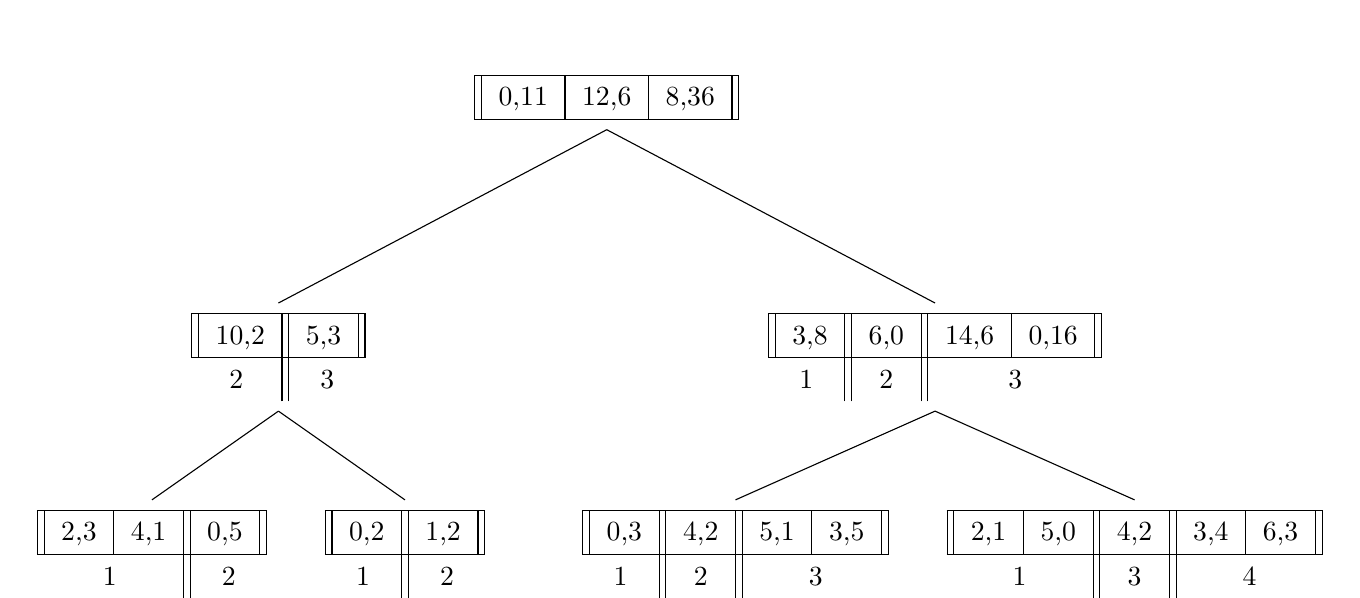
\begin{tikzpicture}[level 1/.style={level distance=3.3cm,sibling distance=1cm},
	level 2/.style={level distance=2.5cm,sibling distance=0.5cm}]
  

\Tree [.{\begin{tabular}{||c|c|c||}  \hline 0,11 & 12,6 & 8,36 \\ \hline\end{tabular}}
 [.{\begin{tabular}{||c||c||}  \hline 10,2 & 5,3 \\  \hline \multicolumn{1}{c||}{2} & \multicolumn{1}{c}{3} \end{tabular}}
 [.{\begin{tabular}{||c|c||c||}\hline 2,3 & 4,1 & 0,5 \\\hline\multicolumn{2}{c||}{1} & \multicolumn{1}{c}{2}\end{tabular}} ]
  [.{\begin{tabular}{||c||c||}  \hline 0,2 & 1,2 \\  \hline \multicolumn{1}{c||}{1} & \multicolumn{1}{c}{2} \end{tabular}} ] ]
          [.{\begin{tabular}{||c||c||c|c||}  \hline 3,8 & 6,0 & 14,6 & 0,16 \\ \hline \multicolumn{1}{c||}{1} & \multicolumn{1}{c||}{2} & \multicolumn{2}{c}{3}\end{tabular}}
           [.{\begin{tabular}{||c||c||c|c||}  \hline 0,3 & 4,2 & 5,1 & 3,5 \\ \hline \multicolumn{1}{c||}{1} & \multicolumn{1}{c||}{2}& \multicolumn{2}{c}{3}\end{tabular}} ]
            [.{\begin{tabular}{||c|c||c||c|c||}  \hline 2,1 & 5,0 & 4,2 & 3,4 & 6,3 \\ \hline \multicolumn{2}{c||}{1} & \multicolumn{1}{c||}{3} & \multicolumn{2}{c}{4}\end{tabular}} ] ] ]

\end{tikzpicture}
\end{center}

\vspace{3em}
\begin{center}
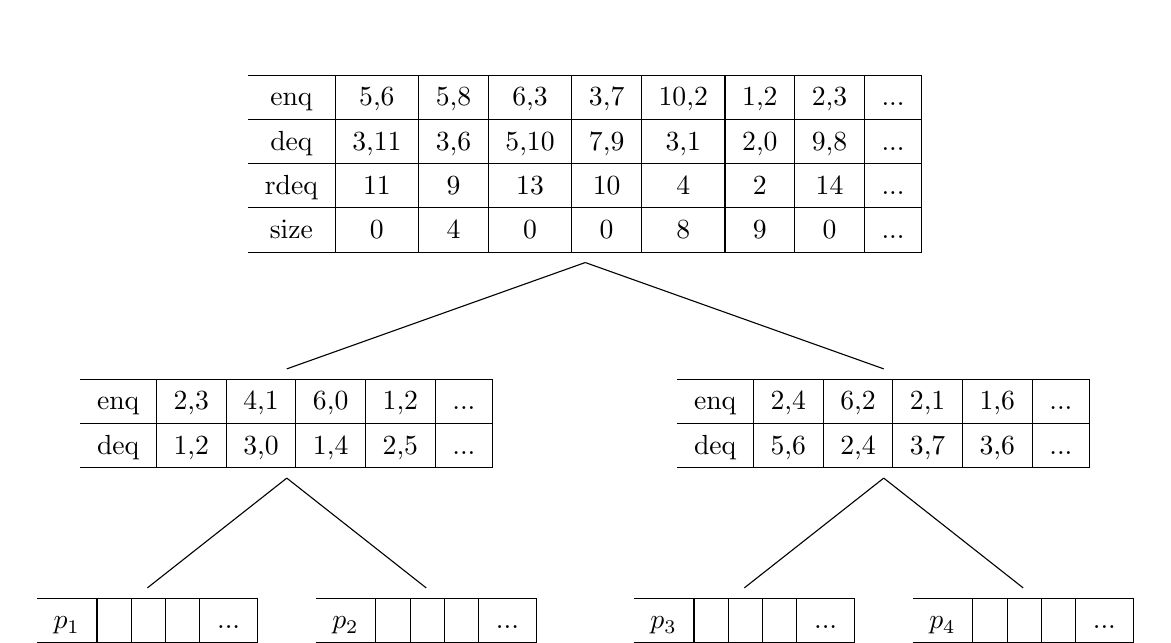
\begin{tikzpicture}[level 1/.style={level distance=3.3cm,sibling distance=1cm},
	level 2/.style={level distance=2.5cm,sibling distance=0.5cm}]
  

\Tree [.{\begin{tabular}{c|c|c|c|c|c|c|c|c|}
    \hline enq & 5,6 & 5,8 & 6,3 & 3,7 & 10,2 & 1,2 & 2,3 & ... \\
    \hline deq & 3,11 & 3,6 & 5,10 & 7,9 & 3,1 & 2,0 & 9,8 & ... \\
    \hline rdeq & 11 & 9 & 13 & 10 & 4 & 2 & 14 & ... \\ 
    \hline size & 0 & 4 & 0 & 0 & 8 & 9 & 0 &... \\ \hline\end{tabular}}
     [.{\begin{tabular}{c|c|c|c|c|c|c|}  \hline enq & 2,3 & 4,1 & 6,0 & 1,2 & ... \\ \hline deq & 1,2 & 3,0 & 1,4 & 2,5 & ... \\ \hline\end{tabular}}
      {\begin{tabular}{c|c|c|c|c|}  \hline $p_1$ & &  & & ... \\ \hline\end{tabular}} {\begin{tabular}{c|c|c|c|c|}  \hline $p_2$ & & & & ... \\ \hline\end{tabular}} ] [.{\begin{tabular}{c|c|c|c|c|c|}  \hline enq & 2,4 & 6,2 & 2,1 & 1,6 & ... \\ \hline deq & 5,6 & 2,4 & 3,7 & 3,6 & ... \\ \hline\end{tabular}} {\begin{tabular}{l|c|c|c|c|}  \hline $p_3$ & & & & ... \\ \hline\end{tabular}} {\begin{tabular}{l|c|c|c|c|}  \hline $p_4$ & & & & ... \\ \hline\end{tabular}} ] ]

\end{tikzpicture}
\end{center}

\question{Description}

In our model each process has an array which it appends its outgoing operation to it. Then there is a shared tournament tree that its leaves are operation lists of processes. Nodes of the tournament tree contain list of blocks. each block is a summarization of the operation propagated together. it has 4 numbers that tell us how many operation from which type has propagated from which child. In each block we order operation by this ordering(enqueus from left child, enqueues from right child, dequeues from left child, dequeues from right child) and by this rule we can find i-th operation type and the child that it has propagated up from.

Propagate procedure: First we create a block of newly added operation to children of the given node, then try to apen it to the last of the block lists. If it fails we try again.



\begin{algorithm}
\caption{Main Algorithm}\label{alg}
\begin{algorithmic}[1]
\onehalfspacing


\Function{Do}{operation op}
\State add p to this.ops
\State \Call{Propagate}{this.ops}
\State \Comment{When is op added to the root?}
\If{op is a deq}
\State before-size: size of the block before block containing op
\State e: \#enqs in the block containing op
\State d: \#deqs in the block containing op before op
\If{before-size + e - d $<$ 1}
\State \Return{null}
\Else{}
\State d: \#rdeqs before the op in all the ordering
\State \Return{enq(d+1)} \#d+1th enq value in all the enqs
\EndIf
\EndIf
\EndFunction
\Statex

\Function{Propagate}{node n}
\State b=\Call{Create-Block}{n}
\If{!\Call{tryAppend}{b, n}}
\Call{tryAppend}{b, n}
\EndIf
\State \Call{Propagate}{n.parent}
\EndFunction
\Statex

\Function{Create-Block}{n}
\Statex \Comment constructs block of the new operation in children of n. if n is root it has extra fields: size, rdeqs.
\EndFunction
\Statex

\Function{tryAppend}{b, n}
\Statex \Comment tries to append b to the last of the n's list.
\EndFunction
\Statex

\Function{Index}{operation op, level $\in$ nodes, type $\in\{$block, operation$\}$}
\Statex \Comment returns index of op in the given level, e.g  Index(op, root, block) return ordering of the block containing op in the root blocks.
\EndFunction
\Statex

\Function{Access}{i, level $\in$ nodes, type $\in\{$enq, deq$\}$}
\Statex \Comment returns i-th operation of given type in the given node subtree.
\EndFunction
\Statex

\Function{Prefix-Sum}{i, level $\in$ nodes, type$\in\{$enq, deq, rdeq$\}$}
\Statex \Comment computes how many of the given type operations are before the ith operation in the given level. For rdeq it will only get root level.
\EndFunction


\end{algorithmic}
\end{algorithm}
\pagebreak


\end{document}




